%$Id: chi06.tex,v 1.4 2006/02/13 23:19:21 rlw Exp rlw $
\documentclass[dvips]{beamer}
\usetheme[hideothersubsections]{Boston}
\usepackage{amsmath,amssymb,bm,array,graphicx,epic,hyperref,url,psfrag}
%\usepackage{movie15}
%\bibliographystyle{jasa}
\graphicspath{{./}{eps/}}
\setbeamercovered{transparent}
\title{Nonparametric Function Estimation }
\subtitle{\Large Using L\'evy Random Field Priors}
\author[M. Clyde]{Merlise Clyde}
\institute{Department of Statistical Science \\ Duke
University }
\date{Joint Statistics  Meeting \\ July 31, 2007}
\newcommand{\bs}[2]{\begin{frame} \frametitle{#1} 
{#2}
\end{frame} }
\usepackage{xcolor}
\definecolor{beamer@blendedblue}{RGB}{86,155,189}
\definecolor{myblue}{RGB}{12,76,138}
\setbeamercolor{structure}{fg=myblue}
\definecolor{Ftitle}{RGB}{12,76,138}
\definecolor{Descitem}{RGB}{238,238,244}
\definecolor{StdTitle}{RGB}{12,76,138}
\definecolor{StdBody}{RGB}{213,24,0}
\definecolor{StdBody}{RGB}{213,24,0}

\definecolor{AlTitle}{RGB}{255, 190, 190}
\definecolor{AlBody}{RGB}{213,24,0}

\definecolor{ExTitle}{RGB}{201, 217, 217}
\definecolor{ExBody}{RGB}{213,24,0}

\setbeamercolor{frametitle}{fg = Ftitle}
\setbeamercolor{title}{fg = Ftitle}
\setbeamercolor{item}{fg = Ftitle}
\setbeamercolor{subitem}{fg = Ftitle}
\setbeamercolor{subsubitem}{fg = Ftitle}
\setbeamercolor{description item}{fg = myblue}
\setbeamercolor{titlelike}{fg=myblue}

%$Id: macros.tex,v 1.2 2006/02/13 14:23:55 rlw Exp rlw $
\newcommand{\Lmea}{{\cal L}} 
\newcommand{\scale}{\bflambda} 
\newcommand{\Scale}{\bfLambda} 
\newcommand{\bfscale}{\bflambda} 
\newcommand{\mean}{\bfchi}
\newcommand{\loc}{\bfchi}
\newcommand{\bfmean}{\bfchi}
\renewcommand{\k}{g}
\newcommand{\Gen}{{\cal G}}
\newcommand{\eps}{\epsilon}

\newcommand{\ind}{\mathrel{\mathop{\sim}\limits^{\mathit{ind}}}}
\newcommand{\iid}{\mathrel{\mathop{\sim}\limits^{\mathit{iid}}}}
\newcommand{\dis}{\mathrel{\mathop{=}\limits^{d}}}
\newcommand{\sgn}{\mathop{\rm sgn}}
\newcommand{\cmp}{h}
\newcommand{\dbdo}{d\beta ~ d\omega}
\newcommand{\real}{{\mathbb{R}}}
\newcommand{\Ber}{\mbox{\rm Ber}}
\newcommand{\GP}{\mbox{\rm GP}}
\newcommand{\SaS}{\text{S$\alpha$S}}
\newcommand{\RA}{{\real \times A}}
\newcommand{\RK}{{\real \times K}}
\newcommand{\RO}{{\real \times \Omega}} 
\newcommand{\RS}{{\bbR \times \LamS}}
  \newcommand{\set}[1]{\left\{#1\right\}}
  \newcommand{\bet}[1]{\left[#1\right]}
  \newcommand{\cet}[1]{\left(#1\right)}
%  \renewcommand{\half}{{\scriptstyle\frac12}}
\newcommand{\subA}{(\eps_1 < \beta \le \eps_2) \times \LamS}
 \newcommand{\uu}{{\big(\scale(x - \loc)\big)}}
 \newcommand{\uuj}{{\big(\scale_j(x-\loc_j)\big)}}
 \newcommand{\bbT}{{\mathbb{T}}}
 \newcommand{\ui}{{[0,1)}}
 \newcommand{\spq}[1]{\left|#1\right|^s_{pq}}
 \newcommand{\spqper}[1]{\left|#1\right|^{s\,*}_{pq}}
 \newcommand{\sspqper}[1]{\left\|#1\right\|^{s\,*}_{pq}}
 \newcommand{\sspq}[1]{\left\|#1\right\|^s_{pq}}    % Besov semi-norm
 \newcommand{\qp}[1]  {\left\|#1\right\|^q_p}         % Hilbert-space norm
 \newcommand{\qper}[1]{\left\|#1\right\|^{*\,q}_p}  % Periodic HS norm
 

\newcommand{\bbW}{{\mathbb{W}}}
\newcommand{\bbB}{{\mathbb{B}}}
\newcommand{\Sob}{{\ensuremath{\bbW^s_2}}}
\newcommand{\Besov}{{\ensuremath{\bbB^s_{pq}}}}
\newcommand{\Besper}{{\ensuremath{\bbB^{s\,*}_{pq}}}}
\newcommand{\Sobx}[1]{{\bbW^{#1}_2}}
\newcommand{\Besovx}[1]{{\bbB^{#1}_2}}
\newcommand{\SN}[1]{\|{#1}\|_\Sob}
% MATH LETTER DEFINITIONS
\newcommand{\Levy}{L{\'e}vy}
\newcommand{\nmathbf}{\bm}
\newcommand{\tabb}[1]{\hspace*{#1\parindent}}
%\newcommand{\G}{{g}}    % Really the same as \GB
\newcommand{\g}{{\phi}} %\newcommand{\g}{{g}}
\newcommand{\GB}{{g}}  
% Roman math Bold face 


\def\bfA{\nmathbf A}
\def\bfB{\nmathbf B}
\def\bfC{\nmathbf C}
\def\bfD{\nmathbf D}
\def\bfE{\nmathbf E}
\def\bfF{\nmathbf F}
\def\bfG{\nmathbf G}
\def\bfH{\nmathbf H}
\def\bfI{\nmathbf I}
\def\bfJ{\nmathbf J}
\def\bfK{\nmathbf K}
\def\bfL{\nmathbf L}
\def\bfM{\nmathbf M}
\def\bfN{\nmathbf N}
\def\bfO{\nmathbf O}
\def\bfP{\nmathbf P}
\def\bfQ{\nmathbf Q}
\def\bfR{\nmathbf R}
\def\bfS{\nmathbf S}
\def\bfT{\nmathbf T}
\def\bfU{\nmathbf U}
\def\bfV{\nmathbf V}
\def\bfW{\nmathbf W}
\def\bfX{\nmathbf X}
\def\bfY{\nmathbf Y}
\def\bfZ{\nmathbf Z}

\def\bfa{\nmathbf a}
\def\bfb{\nmathbf b}
\def\bfc{\nmathbf c}
\def\bfd{\nmathbf d}
\def\bfe{\nmathbf e}
\def\bff{\nmathbf f}
\def\bfg{\nmathbf g}
\def\bfh{\nmathbf h}
\def\bfi{\nmathbf i}
\def\bfj{\nmathbf j}
\def\bfk{\nmathbf k}
\def\bfl{\nmathbf l}
\def\bfm{\nmathbf m}
\def\bfn{\nmathbf n}
\def\bfo{\nmathbf o}
\def\bfp{\nmathbf p}
\def\bfq{\nmathbf q}
\def\bfr{\nmathbf r}
\def\bfs{\nmathbf s}
\def\bft{\nmathbf t}
\def\bfu{\nmathbf u}
\def\bfv{\nmathbf v}
\def\bfw{\nmathbf w}
\def\bfx{\nmathbf x}
\def\bfy{\nmathbf y}
\def\bfz{\nmathbf z}


\def\bfalpha  {\nmathbf \alpha}
\def\bfbeta   {\nmathbf \beta}
\def\bfgamma  {\nmathbf \gamma}
\def\bfdelta  {\nmathbf \delta}
\def\bfepsilon{\nmathbf \epsilon}
\def\bfvareps {\nmathbf \varepsilon}
\def\bfzeta   {\nmathbf \zeta}
\def\bfeta    {\nmathbf \eta}
\def\bftheta  {\nmathbf \theta}
\def\bfiota   {\nmathbf \iota}
\def\bfkappa  {\nmathbf \kappa}
\def\bflambda {\nmathbf \lambda}
\def\bfmu     {\nmathbf \mu}
\def\bfnu     {\nmathbf \nu}
\def\bfxi     {\nmathbf \xi}
\def\bfomicron{\nmathbf \omicron}
\def\bfpi     {\nmathbf \pi}
\def\bfrho    {\nmathbf \rho}
\def\bfsigma  {\nmathbf \sigma}
\def\bftau    {\nmathbf \tau}
\def\bfupsilon{\nmathbf \upsilon}
\def\bfphi    {\nmathbf \phi}
\def\bfpsi    {\nmathbf \psi}
\def\bfchi    {\nmathbf \chi}
\def\bfomega  {\nmathbf \omega}
\newcommand{\nubw}{{\tilde\nu}}  % no longer red!
\def\bfAlpha  {\nmathbf \Alpha}
\def\bfBeta   {\nmathbf \Beta}
\def\bfGamma  {\nmathbf \Gamma}
\def\bfDelta  {\nmathbf \Delta}
\def\bfEpsilon{\nmathbf \Epsilon}
\def\bfZeta   {\nmathbf \Zeta}
\def\bfEta    {\nmathbf \Eta}
\def\bfTheta  {\nmathbf \Theta}
\def\bfIota   {\nmathbf \Iota}
\def\bfKappa  {\nmathbf \Kappa}
\def\bfLambda {\nmathbf \Lambda}
\def\bfMu     {\nmathbf \Mu}
\def\bfNu     {\nmathbf \Nu}
\def\bfXi     {\nmathbf \Xi}
\def\bfOmicron{\nmathbf \Omicron}
\def\bfPi     {\nmathbf \Pi}
\def\bfRho    {\nmathbf \Rho}
\def\bfSigma  {\nmathbf \Sigma}
\def\bfTau    {\nmathbf \Tau}
\def\bfUpsilon{\nmathbf \Upsilon}
\def\bfPhi    {\nmathbf \Phi}
\def\bfPsi    {\nmathbf \Psi}
\def\bfChi    {\nmathbf \Chi}
\def\bfOmega  {\nmathbf \Omega}

% Number math Bold face

\newcommand{\bfzero}{{\nmathbf 0}}
\newcommand{\bfone}{{\nmathbf 1}}

% Estimators

\newcommand{\ttheta}{\tilde{\theta}}
\newcommand{\htheta}{\hat{\theta}}
\newcommand{\tbtheta}{\tilde{\bftheta}}
\newcommand{\hbtheta}{\hat{\bftheta}}
\newcommand{\tomega}{\tilde{\omega}}
\newcommand{\homega}{\hat{\omega}}
\newcommand{\tbomega}{\tilde{\bfomega}}
\newcommand{\hbomega}{\hat{\bfomega}}
\newcommand{\tlambda}{\tilde{\lambda}}
\newcommand{\hlambda}{\hat{\lambda}}
\newcommand{\tblambda}{\tilde{\bflambda}}
\newcommand{\hblambda}{\hat{\bflambda}}


% Calligraphic

\newcommand{\mc}[1]{\ensuremath{\mathcal{#1}}}

\newcommand{\cfA}{\mc{A}}
\newcommand{\cfB}{\mc{B}}
\newcommand{\cfC}{\mc{C}}
\newcommand{\cfD}{\mc{D}}
\newcommand{\cfE}{\mc{E}}
\newcommand{\cfF}{\mc{F}}
\newcommand{\cfG}{\mc{G}}
\newcommand{\cfH}{\mc{H}}
\newcommand{\cfI}{\mc{I}}
\newcommand{\cfJ}{\mc{J}}
\newcommand{\cfK}{\mc{K}}
\newcommand{\cfL}{\mc{L}}
\newcommand{\cfM}{\mc{M}}
\newcommand{\cfN}{\mc{N}}
\newcommand{\cfO}{\mc{O}}
\newcommand{\cfP}{\mc{P}}
\newcommand{\cfQ}{\mc{Q}}
\newcommand{\cfR}{\mc{R}}
\newcommand{\cfS}{\mc{S}}
\newcommand{\cfT}{\mc{T}}
\newcommand{\cfU}{\mc{U}}
\newcommand{\cfV}{\mc{V}}
\newcommand{\cfX}{\mc{X}}
\newcommand{\cfY}{\mc{Y}}
\newcommand{\cfZ}{\mc{Z}}

\newcommand{\bmc}[1]{\ensuremath{\boldsymbol{\mathcal{#1}}}}

\newcommand{\bcfA}{\bmc{A}}
\newcommand{\bcfB}{\bmc{B}}
\newcommand{\bcfC}{\bmc{C}}
\newcommand{\bcfD}{\bmc{D}}
\newcommand{\bcfE}{\bmc{E}}
\newcommand{\bcfF}{\bmc{F}}
\newcommand{\bcfG}{\bmc{G}}
\newcommand{\bcfH}{\bmc{H}}
\newcommand{\bcfI}{\bmc{I}}
\newcommand{\bcfJ}{\bmc{J}}
\newcommand{\bcfK}{\bmc{K}}
\newcommand{\bcfL}{\bmc{L}}
\newcommand{\bcfM}{\bmc{M}}
\newcommand{\bcfN}{\bmc{N}}
\newcommand{\bcfO}{\bmc{O}}
\newcommand{\bcfP}{\bmc{P}}
\newcommand{\bcfQ}{\bmc{Q}}
\newcommand{\bcfR}{\bmc{R}}
\newcommand{\bcfS}{\bmc{S}}
\newcommand{\bcfT}{\bmc{T}}
\newcommand{\bcfU}{\bmc{U}}
\newcommand{\bcfV}{\bmc{V}}
\newcommand{\bcfW}{\bmc{W}}
\newcommand{\bcfX}{\bmc{X}}
\newcommand{\bcfY}{\bmc{Y}}
\newcommand{\bcfZ}{\bmc{Z}}

% Special symbols

\newcommand{\reals}{\mbox{\rm I\kern-.20em R}}
\newcommand{\sreals}{\mbox{\small \rm I\kern-.20em R}}
\newcommand{\LamS}{{\cS^d_+}}

% MATHEMATICAL NOTATION

% Operators

\newcommand{\bg}{\;\bigg\vert\;}
\newcommand{\pr}{\mbox{\rm Pr}}
\newcommand{\D}{\mbox{\rm D}}
\newcommand{\E}{\mbox{\rm E}}
\newcommand{\Mo}{\mbox{\rm Mo}}
\newcommand{\Me}{\mbox{\rm Me}}
\newcommand{\Cov}{\mbox{\rm Cov}}
\newcommand{\Var}{\mbox{\rm Var}}
\newcommand{\Corr}{\mbox{\rm Corr}}
\newcommand{\Q}{\mbox{\rm Q}}

% Distributions
\newcommand{\BeBi}{\mbox{\rm BeBi}}
\newcommand{\Be}{\mbox{\rm Be}}
\newcommand{\Bi}{\mbox{\rm Bi}}
\newcommand{\Br}{\mbox{\rm Br}}
\newcommand{\Ca}{\mbox{\rm Ca}}
\newcommand{\Di}{\mbox{\rm Di}}
\newcommand{\Ex}{\mbox{\rm Ex}}
\newcommand{\Fs}{\mbox{\rm Fs}}
\newcommand{\Ga}{\mbox{\sf G}}
\newcommand{\Ge}{\mbox{\rm Ge}}
\newcommand{\GaGa}{\mbox{\rm GaGa}}
\newcommand{\Hy}{\mbox{\rm Hy}}
\newcommand{\IGa}{\mbox{\rm IGa}}
\newcommand{\IPa}{\mbox{\rm IPa}}
\newcommand{\Lo}{\mbox{\rm Lo}}
\newcommand{\Mu}{\mbox{\rm Mu}}
\newcommand{\N}{\mbox{\rm N}}
\newcommand{\NBi}{\mbox{\rm NBi}}
\newcommand{\NGa}{\mbox{\rm NGa}}
\newcommand{\NWi}{\mbox{\rm NWi}}
\newcommand{\Pa}{\mbox{\rm Pa}}
\newcommand{\Po}{\mbox{\sf P}}
\newcommand{\PoGa}{\mbox{\rm PoGa}}
\newcommand{\Ra}{\mbox{\rm Ra}}
\newcommand{\REx}{\mbox{\rm REx}}
\newcommand{\St}{\mbox{\rm St}}
\newcommand{\Un}{\mbox{\rm Un}}
\newcommand{\Wi}{\mbox{\rm Wi}}

% General Mathematics

\newcommand{\dd}[1]{\,d{#1}}
\newcommand{\barx}{\ensuremath{\bar{x}}}
\newcommand{\comb}[2]{{#1\choose#2}}
\newcommand{\ontop}[2]{{#1\atop#2}}
\newcommand{\h}{{\small\ensuremath{1\over2}}}
\newcommand{\hh}[2]{{\small\ensuremath{#1\over#2}}}

\newcommand{\fn}[1]{\hbox{\textrm{#1}}}
\newcommand{\cred}{\fn{Cr}}
\newcommand\dlim{\mathop{\rm \hbox{$\delta$}lim}}
\newcommand{\goto}{\rightarrow}
\newcommand{\gotoinf}{\rightarrow \infty}

\newcommand{\data}{\ensuremath{\bfx=\{x_1,\ldots,x_n\}}}
\newcommand{\brow}[2]{\ensuremath{\{{#1}_1,\ldots,{#1}_{#2}\}}}
\newcommand{\prow}[2]{\ensuremath{({#1}_1,\ldots,{#1}_{#2})}}

\newcommand{\met}{\thinspace{\rm m}}\newcommand{\km}{\thinspace{\rm km}}
\newcommand{\xbar}{\overline X}%
\newcommand{\xbbar}{\overline{\overline X}}%
\font\ss=cmss12
 \newcommand{\OFP}{(\Omega,\cF,\P)}
 \newcommand{\bbC}{\mathbb{C}}
 \newcommand{\bbF}{\mathbb{F}}
 \newcommand{\bbN}{\mathbb{N}}
 \newcommand{\bbR}{\mathbb{R}}
 \newcommand{\bbX}{\mathbb{X}}
 \newcommand{\bbZ}{\mathbb{Z}}
 \newcommand{\one}[1]{\mathbf{1}_{\{#1\}}}
 \newcommand{\cA}{{\cal A}}
 \newcommand{\cB}{{\cal B}} 
 \newcommand{\cE}{{\cal E}}
 \newcommand{\cF}{{\cal F}}
 \newcommand{\cG}{{\cal G}}
 \newcommand{\cH}{{\cal H}}
 \newcommand{\cM}{{\cal M}}
 \newcommand{\cR}{{\cal R}}
 \newcommand{\cS}{{\cal S}}
 \newcommand{\cT}{{\cal T}}
 \newcommand{\cX}{{\cal X}}
 \newcommand{\cY}{{\cal Y}}
 \newcommand{\cZ}{{\cal Z}}
 \newcommand{\eF}{{\CMcal F}}
 \newcommand{\eG}{{\CMcal G}} 
 \newcommand{\eH}{{\CMcal H}}
 \renewcommand{\P}{{\sf{P}}} 
 \renewcommand{\E}{{\sf{E}}}
 \newcommand{\Ev}{{\sf{Ev}}}%
 \newcommand{\V}{{\sf{V}}} 
 \renewcommand{\Cov}{{\sf{Cov}}}
 %\newcommand{\Be}{\textsf{Be}}
 %\newcommand{\Bi}{\textsf{Bi}}
 %\newcommand{\Ex}{\textsf{Ex}}\newcommand{\Ga}{\textsf{Ga}}
 %\newcommand{\Di}{\textsf{Di}}\newcommand{\Ge}{\textsf{Ge}}
 %\newcommand{\IG}{\textsf{IG}}\newcommand{\Lv}{\textsf{Lv}}
 %\newcommand{\HG}{\textsf{HG}}\newcommand{\MN}{\textsf{MN}}
\newcommand{\NB}{\textsf{NB}}\newcommand{\No}{\textsf{N}}
\newcommand{\LN}{\textsf{LN}}
\newcommand{\Lv}{\mbox{\rm Lv}}
%\newcommand{\Pa}{\textsf{Pa}}
% \newcommand{\Po}{\textsf{Po}}\newcommand{\Un}{\textsf{Un}}
 \newcommand{\argmax}{\textrm{argmax}}
 \renewcommand{\th}{{\ensuremath^{\mbox{\tiny th}}}}
 \newcommand{\nd}{{\ensuremath^{\mbox{\tiny nd}}}}
 \newcommand{\st}{{\ensuremath^{\mbox{\tiny st}}}}
 \newcommand{\ii}{{\ensuremath{\bar{i}}}}% \newcommand{\ii}{{\hat i}}
 \newcommand{\jj}{{\ensuremath{\bar{j}}}}%
 \newcommand{\R}{\texttt{R}}
 \newcommand{\mayeq}{\mathrel{\mathop{=}\limits^?}}
 \newcommand{\pperp}{\mathrel{{\rlap{$~\perp$}\perp\,\,}}}
 \newbox\asbox
 \setbox\asbox=\hbox{\vrule height 15pt depth3.5pt width0pt}
 \def\astrut{\relax\ifmmode\copy\strutbox\else\unhcopy\strutbox\fi}
 \def\Strut{\vrule width0pt height 16pt depth 4pt}%
%\font\tinyss=cmss8 at 8truept % for ^T etc
\newcommand{\tsf}[1]{\textsf{\tiny{#1}}}
\newcommand{\fxa}{\mbox{$f(x\mid\alpha)$}}
\newcommand{\fxt}{\mbox{$f(x\mid\theta)$}}
\newcommand{\fxat}{\mbox{$f(x\mid\alpha,\theta)$}}
\newcommand{\tp}{^{\tsf{T}}}
\newcommand{\as}{\textit{a.s.}}
\newcommand{\ie}{\textit{i.e.{}}}
\newcommand{\etc}{\textit{etc}}
\newcommand{\eg}{\textit{e.g.{}}}%
\newcommand{\half}{{\frac12}}
\newcommand{\Sec}[1]{Section\thinspace(\ref{#1})}
\newcommand{\Thm}[1]{Theorem\thinspace\ref{#1}}
\newcommand{\Cor}[1]{Corollary\thinspace\ref{#1}}
\newcommand{\Eqn}[1]{Equation\thinspace(\ref{#1})}
\newcommand{\Fig}[1]{Figure\thinspace(\ref{#1})}
\newcommand{\Figs}[2]{Figures\thinspace(\ref{#1}) and (\ref{#2})}
\newcommand{\Figab}[2]{Figure\thinspace(\ref{#1}#2)}
\newcommand{\Tab}[1]{Table\thinspace(\ref{#1})}
\newcommand{\jth}{{\ensuremath j^{\mbox{\tiny th}}}}%
\providecommand{\ij}{_{ij}} \newcommand{\ji}[1]{_{ij#1}}%
\newcount\ola \newcount\olb \newcount\olc \newcount\old \newcount\ole
\newcount\och\newcount\level
\newtheorem{cor}{Corollary}
\newtheorem{define}{Definition}
\newtheorem{lem}{Lemma}
\newtheorem{prob}{Problem}
\newtheorem{prop}{Proposition}
\newtheorem{thm}{Theorem}
\def\OL#1{\par\noindent\hangindent=#1\parindent % Outline
  \kern1\hangindent\ignorespaces}%
\def\ol#1{%
    \level=#1
    \ifcase\level
    \ola=0 \olb=0 \olc=0 \old=0 \ole=0\or         % Level 0 (reset)
    \olb=0 \olc=0 \old=0 \ole=0 \advance\ola by 1 % Level 1
    \gdef\olev{\uppercase\expandafter{\romannumeral\ola}} \or
    \olc=0 \old=0 \ole=0 \advance\olb by 1        % Level 2
    \och=64 \advance\och by\olb
    \gdef\olev{\char\och}\or
    \old=0 \ole=0 \advance\olc by 1               % Level 3
    \och=48 \advance\och by\olc
    \gdef\olev{\char\och}\or
    \ole=0 \advance\old by 1                      % Level 4
    \och=96 \advance\och by\old
    \gdef\olev{\char\och}\or
    \advance\ole by 1                             % Level 5
    \gdef\olev{\romannumeral\ole} \or
    \message{Outline depth too deep: #1}\fi
    \ifnum\level>0 \OL\level\llap{\olev.\enspace}\ignorespaces\fi}%
\long\def\comment#1/*#2*/{\endcomment}%
\def\endcomment{\relax}%
%
\makeatletter % Find hours (count1) and minutes (count2) past midnight:
\count1\time \divide\count1 60 \count2=-\count1
\multiply\count2 60 \advance\count2 \time
\edef\now{\two@digits{\the\count1}:\two@digits{\the\count2}}
%\renewcommand\section{\@startsection     % Smaller and sans-serif
%    {section}{1}{\z@}{-3.5ex \@plus -1ex \@minus -.2ex}%
%    {2.3ex \@plus.2ex}{\normalfont\large\bfseries\sffamily}}
%\renewcommand\subsection{\@startsection
%    {subsection}{2}{\z@}{-3.25ex\@plus -1ex \@minus -.2ex}%
%    {1.5ex \@plus .2ex}{\normalfont\large\bfseries\sffamily}}
%\renewcommand\subsubsection{\@startsection
%    {subsubsection}{3}{\z@}{-3.25ex\@plus -1ex \@minus -.2ex}%
%    {1.5ex \@plus .2ex}{\normalfont\normalsize\bfseries\sffamily}}
%\def\@seccntformat#1{\csname the#1\endcsname.\quad} % Add . to sec num's
%\long\def\@makecaption#1#2{%                          Use . not : in cap'ns
%  \vskip\abovecaptionskip
%  \sbox\@tempboxa{#1. #2}%
%  \ifdim \wd\@tempboxa >\hsize
%    #1. #2\par
%  \else
%    \global \@minipagefalse
%    \hb@xt@\hsize{\hfil\box\@tempboxa\hfil}%
%  \fi
%  \vskip\belowcaptionskip}
% BEAMER FIX START
\def\newblock{\beamer@newblock}
% BEAMER FIX END
\makeatother

\def\wbox#1#2#3{{\vcenter{\vbox{\hrule height.#3pt
    \hbox{\vrule width.#3pt height#1pt \kern#2pt \vrule width.#3pt}%
                            \hrule height.#3pt}}}}%
\def\Proof.{\medbreak\noindent{\bf Proof.\enspace}}
\def\qed{{\nobreak\hfill\penalty0\hbox to1truecm{}\nobreak
    \hfill$\wbox634$\par\bigskip}}%

%%
%% This is taken from file `dvipsnam.def',
\definecolor{GreenYellow}   {cmyk}{0.15,0,0.69,0}
\definecolor{Yellow}        {cmyk}{0,0,1,0}
\definecolor{Goldenrod}     {cmyk}{0,0.10,0.84,0}
\definecolor{Dandelion}     {cmyk}{0,0.29,0.84,0}
\definecolor{Apricot}       {cmyk}{0,0.32,0.52,0}
\definecolor{Peach}         {cmyk}{0,0.50,0.70,0}
\definecolor{Melon}         {cmyk}{0,0.46,0.50,0}
\definecolor{YellowOrange}  {cmyk}{0,0.42,1,0}
\definecolor{Orange}        {cmyk}{0,0.61,0.87,0}
\definecolor{BurntOrange}   {cmyk}{0,0.51,1,0}
\definecolor{Bittersweet}   {cmyk}{0,0.75,1,0.24}
\definecolor{RedOrange}     {cmyk}{0,0.77,0.87,0}
\definecolor{Mahogany}      {cmyk}{0,0.85,0.87,0.35}
\definecolor{Maroon}        {cmyk}{0,0.87,0.68,0.32}
\definecolor{BrickRed}      {cmyk}{0,0.89,0.94,0.28}
\definecolor{Red}           {cmyk}{0,1,1,0}
\definecolor{OrangeRed}     {cmyk}{0,1,0.50,0}
\definecolor{RubineRed}     {cmyk}{0,1,0.13,0}
\definecolor{WildStrawberry}{cmyk}{0,0.96,0.39,0}
\definecolor{Salmon}        {cmyk}{0,0.53,0.38,0}
\definecolor{CarnationPink} {cmyk}{0,0.63,0,0}
\definecolor{Magenta}       {cmyk}{0,1,0,0}
\definecolor{VioletRed}     {cmyk}{0,0.81,0,0}
\definecolor{Rhodamine}     {cmyk}{0,0.82,0,0}
\definecolor{Mulberry}      {cmyk}{0.34,0.90,0,0.02}
\definecolor{RedViolet}     {cmyk}{0.07,0.90,0,0.34}
\definecolor{Fuchsia}       {cmyk}{0.47,0.91,0,0.08}
\definecolor{Lavender}      {cmyk}{0,0.48,0,0}
\definecolor{Thistle}       {cmyk}{0.12,0.59,0,0}
\definecolor{Orchid}        {cmyk}{0.32,0.64,0,0}
\definecolor{DarkOrchid}    {cmyk}{0.40,0.80,0.20,0}
\definecolor{Purple}        {cmyk}{0.45,0.86,0,0}
\definecolor{Plum}          {cmyk}{0.50,1,0,0}
\definecolor{Violet}        {cmyk}{0.79,0.88,0,0}
\definecolor{RoyalPurple}   {cmyk}{0.75,0.90,0,0}
\definecolor{BlueViolet}    {cmyk}{0.86,0.91,0,0.04}
\definecolor{Periwinkle}    {cmyk}{0.57,0.55,0,0}
\definecolor{CadetBlue}     {cmyk}{0.62,0.57,0.23,0}
\definecolor{CornflowerBlue}{cmyk}{0.65,0.13,0,0}
\definecolor{MidnightBlue}  {cmyk}{0.98,0.13,0,0.43}
\definecolor{NavyBlue}      {cmyk}{0.94,0.54,0,0}
\definecolor{RoyalBlue}     {cmyk}{1,0.50,0,0}
\definecolor{Blue}          {cmyk}{1,1,0,0}
\definecolor{Cerulean}      {cmyk}{0.94,0.11,0,0}
\definecolor{Cyan}          {cmyk}{1,0,0,0}
\definecolor{ProcessBlue}   {cmyk}{0.96,0,0,0}
\definecolor{SkyBlue}       {cmyk}{0.62,0,0.12,0}
\definecolor{Turquoise}     {cmyk}{0.85,0,0.20,0}
\definecolor{TealBlue}      {cmyk}{0.86,0,0.34,0.02}
\definecolor{Aquamarine}    {cmyk}{0.82,0,0.30,0}
\definecolor{BlueGreen}     {cmyk}{0.85,0,0.33,0}
\definecolor{Emerald}       {cmyk}{1,0,0.50,0}
\definecolor{JungleGreen}   {cmyk}{0.99,0,0.52,0}
\definecolor{SeaGreen}      {cmyk}{0.69,0,0.50,0}
\definecolor{Green}         {cmyk}{1,0,1,0}
\definecolor{ForestGreen}   {cmyk}{0.91,0,0.88,0.12}
\definecolor{PineGreen}     {cmyk}{0.92,0,0.59,0.25}
\definecolor{LimeGreen}     {cmyk}{0.50,0,1,0}
\definecolor{YellowGreen}   {cmyk}{0.44,0,0.74,0}
\definecolor{SpringGreen}   {cmyk}{0.26,0,0.76,0}
\definecolor{OliveGreen}    {cmyk}{0.64,0,0.95,0.40}
\definecolor{RawSienna}     {cmyk}{0,0.72,1,0.45}
\definecolor{Sepia}         {cmyk}{0,0.83,1,0.70}
\definecolor{Brown}         {cmyk}{0,0.81,1,0.60}
\definecolor{Tan}           {cmyk}{0.14,0.42,0.56,0}
\definecolor{Gray}          {cmyk}{0,0,0,0.50}
\definecolor{Black}         {cmyk}{0,0,0,1}
\definecolor{White}         {cmyk}{0,0,0,0}
\endinput
%%
%% End of file `mycolor.tex'.

\newcommand{\blue}{\textcolor{Blue}}
\newcommand{\green}{\textcolor{PineGreen}}
\newcommand{\purple}{\textcolor{Purple}}
\newcommand{\red}{\textcolor{RedOrange}}
\definecolor{aper}{rgb}{0.7412,0,1}
\definecolor{daily}{rgb}{0.1412,0,1}
\newcommand{\ap}{\textcolor{aper}}
\newcommand{\dy}{\textcolor{daily}}
\logo{
\includegraphics[width=.6in,height=.6in]{duke}}


\begin{document}
\begin{frame}
  \titlepage
\end{frame}
%\section[Outline]{}

%\bs{Outline}{
%\tableofcontents 
%}

\section{Nonparametric Regression}
\bs{Problem Setting}{
  \begin{itemize}
  \item  Model:
    \begin{itemize}
    \item Observe data $\{Y_i, \bfx_i\} \quad i = 1, \dots n $
    \item $ \E[Y \mid \bfx] = f(\bfx), \quad \bfx \in \cfX$
    \item Goal: inference about unknown $f(\bfx):  \cfX\to\bbR$\\   
\end{itemize}

\item Prior Distributions on $f$:

\begin{itemize}
\item  Dirichlet and Spatial Dirichlet Process priors
\item  Gaussian Process Priors
\item  Basis Expansions of $f$
\end{itemize}
\end{itemize}
}

\subsection{Expansions}
\bs{Nonparametric Regression} {
Need to place a prior on unknown function $f \in \cfF$


Expansions $f(\bfx_i) = \sum_j  \psi_j(\bfx_i)\beta_j$
   \begin{itemize}
   \item  $\{\psi_j\}$: basis functions for some
     function space $\cfF$ %(\eg, $L^2(\cfX,dx$)) 
   \item  $\{\beta_j\}$  unknown coefficients
   \item Commonly used basis functions:
 \begin{itemize}
 \item Polynomials
 \item Fourier 
 \item Splines 
 \item Kernels 
 \item Wavelets 
 \end{itemize} 
   \end{itemize}

}

\bs{Which Basis Expansion?}
{
  \begin{itemize}
  \item[]<1-> Representations with (orthonormal) bases may be inefficient $\ldots$ \\

\item<1->Canonical  basis:
\[f = \left( \begin{array}{c} 42 \\ 42 \\ 42 \end{array} \right) 
  = 42 \left( \begin{array}{c} 1 \\ 0 \\ 0 \end{array} \right) +
    42 \left( \begin{array}{c} 0 \\ 1 \\ 0 \end{array} \right) +
    42\left( \begin{array}{c} 0 \\ 0 \\ 1 \end{array} \right)\]
\item<2-> Enlarging the \textit{dictionary} with element
    $(1,1,1)'$ allows  parsimony:
\[\hspace{-.5in} f %= \left( \begin{array}{c} 42 \\ 42 \\ 42 \end{array} \right) 
  = 42 \left( \begin{array}{c} 1 \\ 1 \\ 1 \end{array} \right) +
    0 \left( \begin{array}{c} 1 \\ 0 \\ 0 \end{array} \right) +
    0 \left( \begin{array}{c} 0 \\ 1 \\ 0 \end{array} \right) +
    0 \left( \begin{array}{c} 0 \\ 0 \\ 1 \end{array} \right)  +
    0 \left( \begin{array}{c} 1 \\ 1 \\ 0 \end{array} \right)  +
    0 \left( \begin{array}{c} 1 \\ 0 \\ 1 \end{array} \right)  +
    0 \left( \begin{array}{c} 0 \\ 1 \\ 1 \end{array} \right)  
\]
  \end{itemize}

}

\subsection{Over-complete Dictionaries }

\bs{Over-complete Dictionaries (OCD)} {
\begin{itemize}
\item  Collection $\{\psi_{j}(\bfx) \}$  ``more than a basis''
  \item Examples:
    \begin{itemize}
    \item ``Large $p$, small $n$''
    \item Unions of two (or more) bases
    \item Translation Invariant Wavelets
      % $\phi_{j,k}(x) = |a|^{-j/2}\psi\left( \frac{x - k
      %     b}{a^j}\right) \quad j, k, \in \bbZ $;
    \item Free-knot splines
    \item Gabor frames
   % $\psi_{j,k}(x) = e^{2 \pi  i j b x} g( x - k a) \quad  j, k \in \bbZ$  ; 
   \item Kernels:  $\psi_j(\bfx) = k(\bfx; \bfomega)$ or other
     generating functions
   \end{itemize}
\item   Expand $f$ in terms of OCD  
   \[ f(\bfx_i) = \sum_{j \in \cfJ } \psi_j(\bfx_i)\beta_j,\qquad f \in
   \bbF=\overline{\{\psi_{j}\}}\]
  \end{itemize} 
}

\bs{L\'evy Adaptive Regression Kernels} {
Generating function:  $\k(\bfx, \omega): \cfX \times \bfOmega \to \bbR$

\begin{eqnarray*}
\k(x,\bfomega_j) & = & \exp\left(-\scale_j|x-\mean_j|^{\rho_j}\right) \\
f(x) &  = &  \sum_{j\le J}\k(x; \bfomega_j) \beta_j \equiv \int_{\bfOmega}  
\k(x;\bfomega) \Lmea(d\bfomega) \\
\Lmea(d\bfomega) & = &\sum_{j\le J} \beta_j \delta_{\bfomega_j}(d\bfomega)
\end{eqnarray*}

  \begin{itemize}
  
  \item  support points of $\Lmea$: $\{\bfomega_j\} = \{(\mean_j,\scale_j, \rho_j)
     \}$ 
    \begin{itemize}
    \item``location'' of kernel:  $\mean_j\in\cfX$  \blue{(unknown)}
    \item ``scale'' of kernel:  $\scale_j\in\bbR^+$   \blue{(unknown)}
    \end{itemize} 
  \item jump sizes of measure:  $\beta_j$   \blue{(unknown)} 
  \item number of support points  $J$ \blue{(unknown)}
  \end{itemize}
} 

\bs{Kernel Convolution of a Pure Jump Process} {
\begin{figure}[!h]
  \begin{center}
    \includegraphics[angle=270,origin=l,totalheight=6truecm,
     clip=1, width=10cm]{gammaproc2.ps}
  \end{center}
\end{figure}
}

\bs{Why Over-complete Dictionaries?} {
  \begin{itemize}
  \item[$+$] More flexible - local adaptivity
  \item[$+$] Potential for sparse representations
  \item[]
  \item[$-$] Non-unique coefficients
  \item[$-$] Computationally intensive search over (uncountable)
    dictionary 
\item[]
\item[+/-] If we are careful, no need to restrict to proper
  priors (!)  (at least in theory)
\end{itemize}
}


\bs{Model Space with OCDs}{
"Space is big. Really big. You just won't believe how vastly hugely
mind-bogglingly big it is."  -- D. Adams

\vspace{.25in}
\centerline{
\includegraphics[height=2in]{dont-panic}}
}

\subsection{L\'evy Random Field Priors }

\bs{ L\'evy  Random Fields} {
  \begin{itemize}
  \item 
$\Lmea(d\bfomega)$  is a \blue{random (signed) measure} on $\bfOmega$ 

\item Convenient to think of a random measure as stochastic process where
$\Lmea$ assigns random variables  to sets $A \in \bfOmega$

\item Take
$$\Lmea \sim \Lv(\nu) \text{ with L\'evy measure } \nu(d \beta, d
  \bfomega)$$
where $\nu$ satisfies integrability condition:
$$\int_{\bbR \times \Omega} \min(1, \beta^2) \, \nu(d\beta, d
  \bfomega) < \infty$$
  \end{itemize}

\blue{Poisson Representation} of L\'evy Random Fields is the key to
Bayesian Inference!
}

\bs{Poisson Representation}{ 
Goal: $f(x) = \sum_{j < J}  \k(\bfx, \bfomega_j) \beta_j$ 

\blue{Sufficient condition}:
$$\int_{\bbR \times \Omega} \min(1, |\beta|) \nu(d\beta, d
  \bfomega) < \infty$$

\begin{itemize}
\item[$\Rightarrow$] $J \sim \Po(\nu_+)$,\qquad $\nu_+\equiv
  \nu(\bbR\times\bfOmega)$
\item[$\Rightarrow$] $\beta_j,\bfomega_j \mid J \iid \pi(d\beta, d\bfomega)
  \propto \nu(d\beta,d\bfomega)$.
\end{itemize}

\begin{itemize}
  \item Finite number of ``big'' coefficients $|\beta_j|$  
  \item Possibly infinite number of $\beta \in [-\epsilon, \epsilon]$
  \item Jumps $|\beta_j|$ are absolutely summable\footnote{need to add a term to
\blue{``compensate''} the infinite number of tiny jumps that are not
absolutely summable under the more general integrability condition}

  \end{itemize}
}


\bs{L\'evy Measures \& Selected ID Random Fields} {
  \begin{itemize}
  \item Gamma: $\nu( d\beta, d\bfomega ) = \beta^{-1} \exp(-\tau
    \beta) d\beta \ \gamma(d\bfomega) $

$$\blue{\beta_j \iid \Ga(0, \tau) } $$
   
\item Symmetric Gamma: $\nu( d\beta, d\bfomega ) = |\beta|^{-1} \exp(-\tau |\beta|) d\beta \ \gamma(d\bfomega)$

\item Cauchy:   $\nu( d\beta, d\bfomega ) = c |\beta|^{-2} d\beta \
  \gamma(d\bfomega)$

$$ \blue{\beta_j \mid \lambda_j \ind \N(0, 1/\lambda_j) \qquad
    \lambda_j \iid \Ga(1/2, 0)}$$


  \item Stable: $\nu(d\beta, d\bfomega) =  c_\alpha |\beta|^{-(\alpha
       +1)}\ \gamma(d\bfomega)$
$$\blue{\beta_j \mid \lambda_j \ind \N(0, 1/\lambda_j) \qquad
    \lambda_j \iid \Ga(\alpha/2, 0) \quad 0 < \alpha < 2}$$
  \end{itemize}
Provides a generalization of \blue{Generalized Ridge Priors}
to infinite dimensional case
}


\bs{Approximating L\'evy Random Fields} {
In practice, cannot use infinite expansion
\begin{itemize}
 \item The (random) number of support points $\bfomega$ with $\beta$ in $[-\epsilon, \epsilon]^c$ is finite
\item Fix $\epsilon$  (practical significance)
\item Use approximate L\'evy  measure 
$$\nu_{\epsilon}(d\beta, d\bfomega) \equiv \nu(d\beta, d\bfomega)\bfone(|\beta| > \epsilon)$$
\item[$\Rightarrow$] $J \sim \Po(\nu_{\epsilon}^+)$;
  $\nu^+_{\epsilon} = \nu([-\epsilon, \epsilon]^c, \bfOmega)$
\item $\beta_j, \bfomega_j \iid \pi(d\beta, d\bfomega) \equiv \nu_\epsilon(d\beta , d\bfomega)/\nu^+_{\epsilon}$

\item use RJ-MCMC to update $J, \{\beta_j, \bfomega_j\}$
\end{itemize}
}
\bs{Truncated Cauchy} {
\centerline{Restriction  $|\beta| > \epsilon$}
\psfrag{x}{\small{$\beta$}}
\centerline{\includegraphics[width=2.5in,angle=270]{../eps/cauchy1.ps}}
}
\bs{Contours of Log Prior (in $\bbR^2$) -- Penalties} {
\begin{tabular}{ccc}
Normal  & DE  & Cauchy \\
\includegraphics[angle=270,width=1.25in,clip=1]{../eps/L2.ps} &
\includegraphics[angle=270,width=1.25in,clip=1]{../eps/L1.ps} &
\includegraphics[angle=270,width=1.25in,clip=1]{../eps/cauchy.ps}
\end{tabular}
 
\vspace{.25in}
Penalized Likelihood:
$$-\frac{1}{2 \sigma^2} \sum_i\big(Y_i - f(\bfx_i)\big)^2  - (\alpha +
1) \sum_j
\log(|\beta_j|)  - \nu^+_{\epsilon} \ldots $$
}



\section{Examples}

\subsection{Wavelet Test Functions}

\bs{Wavelet Test Functions (SNR = 7)} {
\begin{figure}[!h]
  \begin{center}
    \includegraphics[angle=270,origin=l,totalheight=6truecm,
     clip=1,width=10cm]{wavedata.ps}
  \end{center}
\end{figure}
}

\bs{Kernel Functions}{
\begin{figure}[!h]
  \begin{center}
    \includegraphics[angle=270,origin=l,totalheight=6truecm,
     clip=1,width=10cm]{kerplot.ps}
  \end{center}
\end{figure}
}

\bs{Comparisons of OCD Methods} {
  \begin{itemize}
  \item Translational Invariant Wavelets -- Laplace Priors
    (Johnstone \& Silverman     2005)  
  \item Continuous Wavelet Dictionary -- Compound Poisson with
    Gaussian Priors (Chu, Clyde, Liang 2007)
  \item LARK Symmetric Gamma
  \item LARK Cauchy
  \end{itemize}
Range of Over-complete Dictionaries and Priors
}
\bs{Comparison of Mean Square Error w/ OCDs} {
100 realizations of each function

\centerline{\includegraphics[width=2.5in,angle=270]{mse.eps} }

}

\subsection{Motorcycle Crash Data}
\bs{Motorcycle Crash Data} {
\par
On average, only $\E[J\mid Y]\approx 4$ jumps are needed for fit:\par
\begin{figure}[!h]
  \begin{center}
    \includegraphics[angle=270,origin=l, clip=1,
     totalheight=6truecm,width=10cm]{motorfitted.ps}
  \end{center}
\end{figure}
}

\bs{Posterior on Kernel Power}{
\[\k(x_i; \bfomega) = e^{-\scale_j |x_i - \mean_j|^\rho}\]

\begin{figure}[!h]
  \begin{center}
    \includegraphics[angle=270,origin=l, clip=1,
     totalheight=6truecm,width=10cm]{motor.rho.ps}
  \end{center}
\end{figure}
}


\subsection{Proteomics}
\bs{MALDI-TOF Mass Spectroscopy} {
%\onlySlide*{1}{\vspace{-.2in}\center{\includegraphics[height = 3.5in, width
%  =1.75in, angle = -90]{../eps/real_dat.ps}} \\}

%\onlySlide*{2}{\vspace{-.2in}\center{\includegraphics[height = 3.5in, width
%  =1.75in, angle = -90]{../eps/real_dat_time.ps}} \\}

%\onlySlide*{3}{\vspace{-.2in}
\center{\includegraphics[height = 3.5in, width  =1.75in, angle = -90]{../eps/real_dat_5_75_time_mz.ps}}
%}

\centerline{Proteins correspond to peaks in the spectrogram}
}



\bs{Natural Basis Functions} {
Peaks for a single spectrum often exhibit Gaussian  form in the time domain
where the ``spread'' is primarily induced from initial velocity distribution. 

\begin{itemize}
\item $f(t) = \sum_{j}^J k(t, \bfomega_j) \beta_j $
\item $J$ is the number of kernels (unknown but finite) corresponding to
  the unknown number of proteins (Poisson \textit{a priori\/})
\item $\{\beta_j \}$  concentration  ($\epsilon$-truncated Gamma process)
\item $\bfomega = (\tau, \lambda)$
  \begin{itemize}
  \item $\{\tau_j\}$  Expected TOF of protein (unknown) (Uniform)
  \item $\{\lambda_j\}$ peak width -- determined by prior on resolution    
  \end{itemize}
\end{itemize}
}



\bs{Estimated Spectrum}  {
\begin{center}
  \begin{tabular}[]{l}
\includegraphics[height=2.5in,width=1.in,angle=270]{../eps/ModAvg_allPks.ps}
\\
%&
\includegraphics[height=2.5in,width=1.in,angle=270]{../eps/ModAvg_firstDeriv.ps}
% \\
%\includegraphics[height=2in,width=1.in,angle=270]{../eps/ModAvg_w2.ps} &
%\includegraphics[height=2in,width=1.in,angle=270]{../eps/res_v_p.ps}
 \end{tabular}
\end{center}
  
}

\bs{Multiple Spectra}{ 
Hierarchical Model: Simultaneous
  \begin{itemize}
  \item  Alignment of spectra ($\tau_{ij}$)
   \item Identification of peaks (proteins)
   \item Differential Expression of Proteins Across Groups
  \end{itemize}
Add ``Mark'' to $\bfomega$:   $\{$ \red{Control}, \purple{Shared},
\blue{Disease} $\}$

\vspace{.25in}
Goal: Classification of subjects from biologically relevant features
        (peaks/proteins not valleys)
}

\subsection{Time Series Models}
\bs{Hourly PM$_{10}$ concentration in Maricopa County, AZ} {
\centerline{\bf April 1998 }
\vspace{-8mm}
\begin{figure}[!h]
  \begin{center}
    \includegraphics[angle=270,origin=l, clip=1,
     totalheight=5truecm,width=10cm]{30daypm10.ps}
  \end{center}
\end{figure}
The ``Spiky'' concentration profiles don't fit ARMA well.
Semi-periodic with possible daily and meteorologically driven patterns.
}
\bs{Marked L\'evy model}{
\begin{eqnarray*}
    Y_{t_i} &=& f(t_i) + \epsilon_i, %\qquad i = 1,2,\cdots, n,
                                      \quad \epsilon_i \iid \N(0, \sigma^2)\\
        f(t) &=& b_0 +   \int_{\bfOmega} k(t;\bfomega)\,\Gamma(d\bfomega)\quad
                                     \red{\swarrow~\textrm{Marks}}\\
      \bfOmega &=& [0,720] \times \bbR_+\times \red{\{0,1\}}\\
%     \bfOmega &=& [0,720] \times \bbR_+\times \red{\{0\}}\cup 
%                [0,24]  \times \bbR_+\times \red{\{1\}}\\
%  k\big(t;(\tau,\lambda,\red0)\big) &=&  e^{-\lambda |t-\tau|}
%  \textrm{\hspace{20mm} \textit{Aperiodic} part}\\
%  k\big(t;(\tau,\lambda,\red1)\big) &=&  e^{-\lambda |(t-\tau)\pmod{24}|}
%  \textrm{\hspace{5mm} \textit{Daily} part}
   k(t;\bfomega) &=&  k\big(t;(\tau,\lambda,\red a)\big)\\
               &=&  \begin{cases}
                     e^{-\lambda |t-\tau|}&\red{a=0},
                       \textrm{\qquad \textit{Aperiodic} part}\\
                     e^{-\lambda |(t-\tau)\pmod{24}|}&\red{a=1},
                       \textrm{\qquad \textit{Daily} part}
                    \end{cases}
\end{eqnarray*}
}


\bs{The Fitted Model} {
\begin{figure}[!h]
  \begin{center}
    \includegraphics[angle=270,origin=l,totalheight=6truecm,
     clip=1,width=10cm]{30daypm10fitted.ps}
  \end{center}
\end{figure}
}


\bs{The Fitted Model: Daily Part} {
\begin{figure}[!h]
  \begin{center}
    \includegraphics[angle=270,origin=l,totalheight=6truecm,
     clip=1,width=10cm]{pm10onefit.daily.ps}
  \end{center}
\end{figure}
}
\bs{The Fitted Model: Predictions} {
\begin{figure}[!h]
  \begin{center}
    \includegraphics[angle=270,origin=l,totalheight=6truecm,
     clip=1,width=10cm]{5daypm10pred.ps}
  \end{center}
\end{figure}
}

\subsection{Multidimensional Time Series}
\bs{Two Pollutants: PM$_{10}$ and CO} {
\begin{figure}[!h]
  \begin{center}
    \includegraphics[angle=270,origin=l,totalheight=6truecm,
     clip=1,width=10cm]{30daypm10co.ps}
  \end{center}
\end{figure}
}
\bs{Marks} {
\red{six marks}
\[ \bfOmega = [0,720] \times \bbR_+ \times \red{\cA},
\qquad \red{\cA\equiv\{0,1,2,3,4,5\}} \]
where
\[ \red a = \begin{cases}
        \red0&\textrm{Aperiodic, PM$_{10}$ (only)}\\
        \red1&\textrm{Daily, PM$_{10}$ (only)}\\
        \red2&\textrm{Aperiodic, CO (only)}\\
        \red3&\textrm{Daily, CO (only)}\\
        \red4&\textrm{Aperiodic, PM$_{10}$ \textit{and} CO}\\
        \red5&\textrm{Daily, PM$_{10}$ \textit{and} CO}
\end{cases}\]
}
\bs{Fits and Predictions: PM$_{10}$ and CO} {
\begin{figure}[!h]
  \begin{center}\vspace{-5mm}
    \begin{tabular}{c}
      \includegraphics[height=45mm, clip=1, angle=270]{30jointpm10fitted.ps}
      \includegraphics[height=45mm, clip=1, angle=270]{5dayjointpredpm10.ps}\\
      \includegraphics[height=45mm, clip=1, angle=270]{30jointcofitted.ps}
      \includegraphics[height=45mm, clip=1, angle=270]{5dayjointpredco.ps}
    \end{tabular}
  \end{center}
\end{figure}
}
\bs{Decomposition, PM$_{10}$} {
\begin{figure}[!h]
  \begin{center}
    \includegraphics[angle=270,origin=l,totalheight=6truecm,
     clip=1,width=10cm]{30dayjointdecpm10.ps}
  \end{center}
\end{figure}
}
\bs{Decomposition, CO} {
\begin{figure}[!h]
  \begin{center}
    \includegraphics[angle=270,origin=l,totalheight=6truecm,
     clip=1,width=10cm]{30dayjointdecco.ps}
  \end{center}
\end{figure}
}

\subsection{LARK Space-Time Models}
\bs{Sulfur Dioxide Concentrations in PA, MD, NJ:} {
\vspace{-8mm}
\begin{figure}[!h]
  \begin{center}
    \includegraphics[angle=270,origin=l, clip=1,
     totalheight=6truecm]{SO2-rlw.ps}
  \end{center}
\end{figure}
\vspace{-5mm}
EPA SO${_2}$ Monitoring stations  are shown as \red{$\Delta$}'s,
Point Sources (power plants, \etc.) as \blue{$+$}'s
}




\section{Summary}
\bs{L\'evy Adaptive Regression  Kernel
  Features} {
  \begin{itemize}
  \item Limit of finite dimensional priors (GRP \& SVSS)
  \item Flexible generating functions (non-parametric)
  \item Kernel \blue{locations} and \blue{shapes} both \blue{adaptive}
  \item Sparse representations
  \item Modelling Dependence 
    \begin{itemize}
    \item[within:] Kernel ``decay''
    \item[across:] Shared jumps
    \end{itemize}
    \item Expressions for Means \& Covariances
    
  \end{itemize}
}
\bs{Features} {
  \begin{itemize}
  \item Non-Gaussian prior and likelihoods -- no need to transform for
  non-negative functions
  \item Interpretation of model parameters \& informative prior
  distributions

  \item Computationally tractable as coefficients updated individually
    or in small blocks -- no need to invert large matrices
  \item Missing observations, irregular space and time,  non-stationarity
  \end{itemize}
}



\bs{Ongoing Work \& Extensions} {
  \begin{itemize}
  \item Other L\'evy processes ($\alpha$-Stable)
  \item Functional Data Analysis
  \item Arbitrary $\cfX$ (higher dimensions)  
  \item Kernel Selection
  \item Multivariate processes  
  \item Theoretical properties (consistency)
  \end{itemize}
}
\bs{Thanks!} {
\begin{center}
Many thanks to Robert Wolpert and Feng Liang \\
and \\
PhD students Jen-Hwa
Chu, Leanna House, Natesh Pillai, \\ Zhi Ouyang, and Chong Tu!
\end{center}
\vspace{.5in}
More details and related work are available at
\centerline{\blue{ \texttt{www.stat.duke.edu}}}
or on request from 
\centerline{\blue{\texttt{clyde@stat.duke.edu}}} \\
\centerline{\blue{\texttt{rlw@stat.duke.edu}}} 
}

%\frame{\bibliography{rw}}
\end{document}
